\documentclass{article}
\usepackage[utf8]{inputenc}
\usepackage{graphicx}
\usepackage{amsmath}
\usepackage[a4paper, margin=1in]{geometry}
\title{Homework 6}
\author{Steve Gillet}
\date{\today}

% Custom information
\newcommand{\className}{Course: Algorithmic Motion Planning – ASEN 5254-001 – Fall 2024}
\newcommand{\professorName}{Professor: Morteza Lahijanian}
\newcommand{\taName}{Teaching Assistant: Yusif Razzaq}

\begin{document}

% Title
\maketitle
\begin{center}
    \large{\className} \\
    \large{\professorName} \\
    \large{\taName}
\end{center}

\section{Exercise 1}

\textbf{(a)} Below is the plot generated by the wavefront algorithm showing the path taken by the point robot:

\begin{figure}[h]
    \centering
    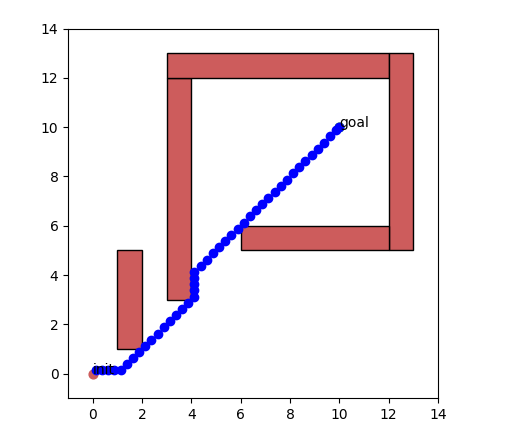
\includegraphics[width=0.8\textwidth]{pointWaveWorkspace.png}
    \caption{Wavefront Path Planning Workspace}
    \label{fig:wavefrontWork}
\end{figure}

Below is the plot genereated by the wavefront algorithm in Cspace:

\begin{figure}[h]
    \centering
    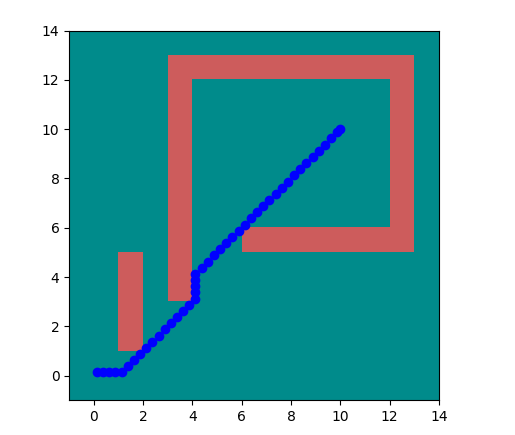
\includegraphics[width=0.8\textwidth]{pointWaveCspace.png}
    \caption{Wavefront Path Planning C-Space}
    \label{fig:wavefrontCspace}
\end{figure}

The robot traverses adjacent cells by connecting the centers of the cells. The wavefront algorithm propagates from the goal and marks cells based on their distance from the goal. The path is generated by following the gradient towards the goal.

\textbf{(b)} The length of the paths can be calculated as the number of cells traversed, multiplied by the grid size. Given that the grid size is $0.25$, the total path length for the point robot is:
\[
\text{Path Length} = n \times 0.25
\]
where $n$ is the number of cells traversed.

For the given plot, $n$ is approximately \(45\), so:
\[
\text{Path Length} \approx 45 \times 0.25 = 11.25 \text{ units}
\]

\textbf{(d)} Yes, we would expect the path length to get smaller as the grid size gets smaller. This is because finer grids allow for more accurate representations of obstacles and paths, leading to more direct routes.

\textbf{(e)} Compared to the gradient descent planner from Homework 5, the wavefront planner offers a more complete exploration of the space. While the gradient descent method relies on local information and can get stuck in local minima, the wavefront method performs a global search and guarantees finding a path (if one exists). There also seems to be a similarity in the challenge of preventing both algorithms from hugging obstacles too closely. Extra care has to be taken to buffer the obstacles because both algorithms will cut as closely to them as their respective functions allow them to.
    

\section{Exercise 2}
\textbf{Problem Statement:} Use the wavefront planner from Exercise 1 to plan a motion for the robotic manipulator in Exercise 3 of Homework 4. The end-effector moves from \( x_{\text{start}} = (-2, 0) \) to \( x_{\text{goal}} = (2, 0) \) in the workspace. Plot the motion in both the C-space and the workspace, showing the computed motion in a series of snapshots.

\textbf{Plot of the Motion Plan:}

\begin{figure}[h]
    \centering
    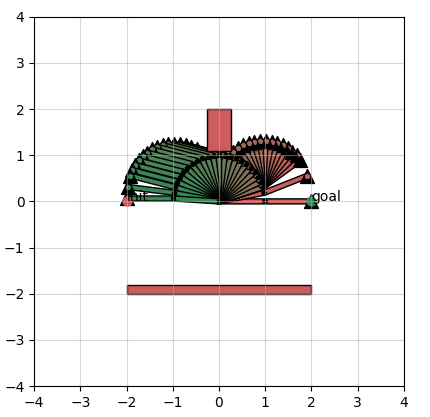
\includegraphics[width=0.8\textwidth]{manipulatorWorkspace.png}
    \caption{Motion of the robotic manipulator from start to goal in workspace}
    \label{fig:manipulatorWorkspace}
\end{figure}

\begin{figure}[h]
    \centering
    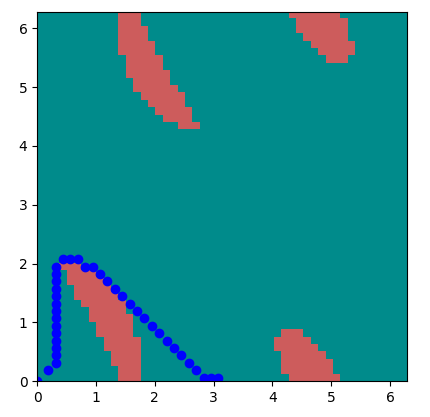
\includegraphics[width=0.8\textwidth]{manipulatorCspace.png}
    \caption{Motion of the robotic manipulator from start to goal in C-space}
    \label{fig:manipulatorCspace}
\end{figure}

The wavefront planner successfully plans the motion for the manipulator. The plot shows the computed motion plan in the robot’s configuration space (C-space) and a series of snapshots of the manipulator's motion in the workspace.

\textbf{Details of the Motion:}
- The wavefront algorithm generates a path from the start configuration to the goal configuration by marking the grid cells and backtracking to create the final path.
- The robot’s end-effector traverses from the initial position at \( (-2, 0) \) to the goal position at \( (2, 0) \) while avoiding obstacles in the workspace.
- The C-space plot highlights how the joint configurations avoid collisions with the obstacles in the workspace.

\section{Exercise 3}

\subsection{Part (a)}
Find the shortest path from $v_{\text{start}} = v_0$ to $v_{\text{goal}} = v_{13}$ in the graph shown in Figure 1 using your A* implementation. Report the path, path length, and number of iterations it took to find this path.

Using A* algorithm, the path from $v_0$ to $v_{13}$ is:
\[v_0 \to v_2 \to v_1 \to v_6 \to v_7 \to v_{13}\]
The total path length is $4$. The number of iterations is unknown.

\subsection{Part (b)}
How can you turn your A* search implementation into Dijkstra's?

\textbf{Answer:}

To turn the A* search implementation into Dijkstra's algorithm, simply set the heuristic value $h(n)$ to $0$ for all nodes $n$. By doing so, A* will no longer prioritize nodes based on an estimated cost to the goal, and instead will explore nodes purely based on the current path cost, which is exactly how Dijkstra's algorithm operates.


\subsection{Part (c)}
Solve the example using Dijkstra's algorithm. Report the path, path length, and the number of iterations it took to find this path.

Using Dijkstra's algorithm, the path from $v_0$ to $v_{13}$ is:
\[v_0 \to v_3 \to v_9 \to v_{13}\]
The total path length is $7$, and it took $6$ iterations to find this path.

\subsection{Part (d)}
Between A* and Dijkstra's algorithm, which one performs better? Which one would you choose to search a large graph for the shortest path between:

\begin{itemize}
    \item [(i)] $v_{\text{start}}$ and $v_{\text{goal}}$
    \item [(ii)] $v_{\text{start}}$ and every $v \in V$
\end{itemize}

\textbf{Answer:}

A* generally performs better when searching for a specific goal node because it uses a heuristic to guide the search, which often reduces the number of nodes that need to be expanded, especially in large graphs with sparse connections. It is most effective when the heuristic is admissible and consistent, allowing A* to find an optimal path with fewer explored nodes.

On the other hand, Dijkstra's algorithm is better suited when finding the shortest paths from $v_{\text{start}}$ to every other node in the graph, as it systematically explores all nodes and ensures that every path is the shortest possible without relying on a heuristic.

- For the shortest path between $v_{\text{start}}$ and $v_{\text{goal}}$, I would choose \textbf{A*}, assuming an appropriate heuristic is available.
- For finding the shortest paths from $v_{\text{start}}$ to every other node ($v \in V$), \textbf{Dijkstra's algorithm} would be more appropriate.

\subsection{Part (e)}
How would you modify your implementation for a graph that is undirected?

\textbf{Answer:}

To modify the implementation for an undirected graph, you need to ensure that each edge is bidirectional. This means that if there is an edge from node $u$ to node $v$, then there must also be an edge from node $v$ to node $u$ with the same weight. This can be achieved by:

1. Adding both directions when defining the edges: for every edge $(u, v, w)$ in the graph, also add $(v, u, w)$.
2. When iterating through the neighbors of a node, both directions will automatically be included, ensuring that the graph is treated as undirected.

In the code, this could be done by modifying the graph construction logic to insert both $(u, v)$ and $(v, u)$ into the adjacency list when adding an edge.


\end{document}
